\documentclass{article}

\usepackage{arxiv}

\usepackage[utf8]{inputenc} % allow utf-8 input
\usepackage[T1]{fontenc}    % use 8-bit T1 fonts
\usepackage{hyperref}       % hyperlinks
\usepackage{url}            % simple URL typesetting
\usepackage{booktabs}       % professional-quality tables
\usepackage{amsfonts}       % blackboard math symbols
\usepackage{nicefrac}       % compact symbols for 1/2, etc.
\usepackage{microtype}      % microtypography
\usepackage{lipsum}		% Can be removed after putting your text content
\usepackage{amssymb,amsmath,amsthm}
\usepackage{listings}
\usepackage{graphicx}
\usepackage{subfig}
\usepackage{apacite}
\usepackage{algorithm}
\usepackage{algorithmicx}
\usepackage{algpseudocode}
\usepackage{kbordermatrix}% http://www.hss.caltech.edu/~kcb/TeX/kbordermatrix.sty
\usepackage{todonotes}
\usepackage{natbib}

\newtheorem{theorem}{Theorem}
\DeclareMathOperator\supp{supp}

\title{Data assimilation with agent-based models using Markov chain sampling}

%\date{September 9, 1985}	% Here you can change the date presented in the paper title
%\date{} 					% Or removing it

\author{
  Daniel Tang\\
    Leeds Institute for Data Analytics, University of Leeds, UK\thanks{This project has received funding from the European Research Council (ERC) under the European Union’s Horizon 2020 research and innovation programme (grant agreement No. 757455)}\\
  \texttt{D.Tang@leeds.ac.uk}\\
  \AND
  Nick Malleson\\
  School of Geography, University of Leeds, UK\\  
  %% examples of more authors
  %% \AND
  %% Coauthor \\
  %% Affiliation \\
  %% Address \\
}


\begin{document}
\maketitle

\begin{abstract}
Every day, weather forecasting centres around the world receive noisy, incomplete observations of the atmosphere and use this data, along with their atmospheric models, to update their beliefs about the state of the atmosphere and their forecasts. This process is known as data assimilation, data fusion or state estimation and is best expressed as Bayesian inference: given a set of observations, some prior beliefs and a model of the target system, what is the probability distribution of some set of unobserved measures at some time, possibly in the future?

While data assimilation has developed rapidly in weather forecasting and other areas, relatively little progress has been made in performing data assimilation with agent based models. This has hampered the use of agent based models to make quantitative claims about real-world systems.

Here we present an algorithm that uses Markov-Chain-Monte-Carlo methods to generate samples of the trajectories of an agent based model over a window of time given a set of noisy, incomplete observations of the system. We demonstrate the algorithm by performing data assimilation with an agent-based, spatial predator-prey model.
\end{abstract}

% keywords can be removed
\keywords{Data assimilation, Bayesian inference, Agent based model, Integer linear programming, predator prey model}

\section{Introduction}

Agent-based models (ABMs) have been widely adopted as an intuitive way to model systems that consist of a heterogeneous collection of autonomous, interacting agents. For example, an ABM of a colony of ants would model each individual ant as an ``agent'' (objects in the environment may also be modelled as agents). ABMs are sometimes used to show that an unexpected collective behaviour can emerge from a given agent behaviour.  For example \citet{schelling1971dynamic} famously showed that agents with only a very slight preference to live close to agents of their own race can quickly form a highly racially-segregated population. This use of ABMs requires no assimilation of real-world data but that means we cannot transfer the model results to the real world without first demonstrating that the model is a proper abstraction of the real-world target system. In this paper, we'll deal with the case where we have an ABM of some real-world target system and some observations of that same system. Our aim will be to combine the information in the observational data with the knowledge embodied in the model to learn something about some set of unobserved measures.

The observations may contain aggregated or macro-scale measures and may be subject to noise during the measurement process. The unobserved measures may span any time interval, and may include times before, during or after the observed interval. The behaviour of the agents in the model will generally be stochastic, in order to account for our uncertainty in agent behaviour, and will be a function of some set of parameters, $\theta$, in order to account for our uncertainty over which behavioural model best represents the real-world target entities, or over the values of measures that are constant through time. Note that the parameters can, and generally should, contain parameters that control the size of the model error. The target system may also interact with a world outside of the model, these interactions necessarily consist of agents being injected into the model at certain times and/or external influences on modelled agent's behaviour\footnote{we take the purist view that an ABM models everything as an agent}. The start state of the model is also a boundary condition, consisting of the injection of agents into the model at time $t=0$. Although the boundary conditions are semantically distinct from the parameters, their mathematical treatment will be identical so we assume $\theta$ includes any boundary conditions. So, an ABM defines a distribution, $P(\tau_t| \theta)$, which is the probability that the agents would exhibit behaviours $\tau_t$ in the time interval $[0,t]$ of a model execution with parameters and boundary conditions $\theta$. We'll call $\tau_t$ a \textit{model trajectory}.

Letting $\Omega$ be our set of real-world observations, we can use Bayes' rule to define what we ought to believe about the joint distribution of model trajectories and parameters given the model and observations
\begin{equation}
P(\tau_t,\theta|\Omega) = \frac{P(\Omega|\tau_t)P(\tau_t|\theta)P(\theta)}{P(\Omega)}
\label{bayesassimilation}
\end{equation}
where $P(\theta)$ is our prior beliefs about the parameters and boundary conditions (after accounting for any micro-calibration data or other relevant observations we may have), $P(\tau_t|\theta)$ is our ABM and $P(\Omega|\tau_t)$ is the probability of making observations $\Omega$ given the trajectory, we assume it is well defined and easy to calculate for some sufficiently large $t$. Finally, the prior probability of the observations, $P(\Omega)$, is just a normalising constant and is not usually explicitly calculated but is dealt with by ensuring any distribution of interest is properly normalised.

Now, if we can generate samples $\left\{\left<\tau_{t1},\theta_1\right> \dots \left<\tau_{tn},\theta_n\right> \right\}$ from $P(\tau_t,\theta|\Omega)$, then we can also generate samples $\left\{\Lambda(\tau_{t1},\theta_1) \dots \Lambda(\tau_{tn},\theta_n) \right\}$ which are draws from $P(\Lambda|\Omega)$, the distribution of the unobserved measures given our observations, which is what we're after. This assumes that $\Lambda$ can be calculated from the model trajectory, the parameters and the boundary conditions\footnote{If this isn't the case then we're simply using the wrong model for our needs}. 

If $P(\theta)$ is in a form that we can sample from then we can, in theory at least, sample from $P(\tau_t,\theta|\Omega)$ by using a simple rejection sampling algorithm as follows
\begin{enumerate}
\item Take a sample from the prior parameters and boundary conditions $\theta' \sim P(\theta)$
\item Execute the model forward with parameters $\theta'$ for time $t$ to generate a sample trajectory $\tau_t' \sim P(\tau_t|\theta')$
\item Accept the sample $\left<\tau_t',\theta'\right>$ with probability $P(\Omega|\tau_t')$ otherwise reject the sample.
\item Repeat until the desired number of samples have been accepted. 
\end{enumerate}

The probability that a sample is accepted is the expectation value of $P(\Omega|\tau_t)$ over $P(\tau_t) = \int P(\tau_t|\theta)P(\theta) d\theta$. But
\[
\mathbb{E}_{P(\tau_t)}(P(\Omega|\tau_t)) = \int P(\Omega|\tau_t)P(\tau_t) d\tau_t = \int P(\Omega|\tau_t) \int P(\tau_t|\theta)P(\theta) d\theta d\tau_t = P(\Omega)
\]
so if the prior probability of the observation, $P(\Omega)$, is sufficiently high then this algorithm will work. However, in practice $P(\Omega)$ is often so low that a rejection sampler would take many years to generate just one sample.

One strategy to tackle this problem is to split the time period $[0,T]$ into smaller, contiguous time windows with (not necessarily equidistant) end times $\left<t_1 \dots t_N\right>$ such that $t_m < t_{m+1}$ and $t_N = T$. The trajectory and observations can be similarly split based on which window they occur in, $\tau_t = \left<\tau^1 \dots \tau^N\right>$ and $\Omega = \left<\Omega_1 \dots \Omega_N\right>$ (windows are often chosen so that there is only a single observation in each window). Equation \eqref{bayesassimilation} can then be split into the product of contributions from each window given the end state from the previous window, leading to a recursion relation
\begin{equation}
P\left(\tau^{1:m+1}, \theta | \Omega_{1:m+1}\right)
=
\frac{ P(\Omega_{m+1}|\tau^{m+1})P(\tau^{m+1}|\theta^{t_m}(\tau^m,\theta))}
{	P(\Omega_{m+1}| \Omega_{1:m}) }
P\left(\tau^{1:m},\theta| \Omega_{1:m}\right)
\label{bayesrecursion}
\end{equation}
where $\theta^{t_m}(\tau^m,\theta)$ gives the parameters/boundary conditions for a simulation that starts at time $t_m$ with a start state given by the state at the end of $\tau^m$ and other parameters/boundary conditions given by $\theta$. This recursion helps in two respects, firstly the dimension of the distributions we need to deal with are reduced since we're only concerned with the trajectory in one window at a time, secondly we've replaced the prior of all observations $P(\Omega)$ with the probability of the observations in a single window, given the previous observations $P(\Omega_{m+1}|\Omega_{1:m})$ meaning that it's easier to find a forecast $\tau^{m+1}$ with non-zero posterior probability. This describes the \textit{particle filtering} or \textit{sequential Monte Carlo} approach to Bayesian inference.

If we let $\sigma^m$ be the state of the model (i.e. the states of all agents) at time $t^m$ and marginalise equation \eqref{bayesrecursion} over $\tau^{1:m+1}$ for a fixed $\sigma^{m+1}$ then we get an alternative recursion
\begin{equation}
P\left(\sigma^{m+1}, \theta | \Omega_{1:m+1}\right)
=
\frac{ P(\Omega_{m+1}|\sigma^{m+1})}
{	P(\Omega_{m+1}| \Omega_{1:m}) }
\int P(\sigma^{m+1}|\theta^{t_m}(\sigma^m,\theta))P\left(\sigma^{m},\theta| \Omega_{1:m}\right) d \sigma^m
\label{bayesstaterecursion}
\end{equation}
where we've assumed that the observation likelihood in window $m+1$ only depends on the model state at time $t^{m+1}$ and made explicit that $\theta^{t_m}(\sigma^m,\theta)$ depends only on $\theta$ and the model state at time $t^m$.  If the unobserved measures of interest, $\Lambda$, depend only on $\left<\sigma^N,\theta\right>$, rather than on the full trajectory, $\left<\tau^{1:N},\theta\right>$, then we can solve this recursion instead, which reduces the dimensionality still further. Note that the definition of ``model state'' can always be re-defined in such a way as to make these assumptions true.

This recursion effectively splits the problem into a number of sub-problems of the form: given a set of samples $\left\{T^m_0 \dots T^m_S\right\}$, where $T^m=\left<\sigma^m,\theta\right>$, which are drawn from $P(\sigma^m,\theta|\Omega_{1:m})$, generate a set of samples  $\left\{T^{m+1}_0 \dots T^{m+1}_S\right\}$ drawn from $P(\sigma^{m+1},\theta|\Omega_{1:m+1})$ as defined by equation \eqref{bayesstaterecursion}.  

This recursion can be implemented in practice with a simple algorithm known as sequential importance resampling which consists of the following steps
\begin{enumerate}
\item generate a set of samples $\left\{T^0_0 \dots T^0_S\right\}$ from the prior $P(\sigma^0,\theta)$. Set $m=0$

\item for each sample $T^m_i = \left<\sigma^m_i,\theta_i\right>$, generate a sample from $\sigma^{m+1}_i \sim P(\sigma^{m+1}|\theta^{t_m}(\sigma^m_i,\theta_i))$ by executing the ABM from the end state of the previous window to create a forecast $T^{m+1}_i = \left<\sigma^{m+1}_i,\theta_i\right>$

\item Turn the forecast into an importance sample from the posterior by assigning a weight to each $T^{m+1}_i$
\[
w_i = \frac{P(\Omega_{m+1}|\sigma^{m+1}_i)}{\sum_{j=0}^S P(\Omega_{m+1}|\sigma^{m+1}_j)}
\]

\item Resample from the posterior by taking $S$ samples from the importance sampling approximation
\begin{equation}
P(\tau^{0:m+1},\theta|\Omega_{0:m+1}) \approx  \sum_i w_i\delta_{\tau^{0:m+1}_i}\left(\tau^{0:m+1}\right)\delta_{\theta_i}(\theta)
\label{importanceApprox}
\end{equation}
where $\delta$ is the delta function. There are a few ways of doing this \citep{douc2005comparison}, the simplest being to choose an integer $i\in[0,S]$ with probability $w_i$, returning the sample $T^{m+1}_i$ and repeating $S$ times.

\end{enumerate}

However, this algorithm suffers from the problem of \textit{sample impoverishment} \citep{li2014fight} or \textit{sample deprivation} which describes the situation when the resampling step leaves many particles in the same state, so the number of distinct samples in our sample set is much smaller than the number of samples. \citet{chatterjee2018sample} show that at each importance sampling step the effective sample size reduces exponentially with the KL-divergence from the forecast to the posterior, $D_{KL}\left(P(\tau^{m+1},\theta|\Omega_{0:m+1}) \mid\mid P(\tau^{0:m+1},\theta|\Omega_{0:m})\right)$, so if the observation $\Omega_{m+1}$ contains a lot of information, which it often does, then we should expect the weighted samples to have an effective sample size much smaller than $S$ and the resampling step to cause some impoverishment. In the worst case, $\Omega_{m+1}$ is an impossible observation for all our samples up to $t_m$ and we end up with an effective sample size of zero. \citet{malleson_simulating_2020} show that sample impoverishment is an issue in practice when applied to data assimilation with an ABM of crowd movement.

To get a better understanding of impoverishment, consider a set of samples of the full trajectory $\left\{\left<\tau^{1:N}_0,\theta_0\right> \dots \left<\tau^{1:N}_S,\theta_S\right>\right\}$ taken from $P(\tau^{1:N},\theta|\Omega_{1:N})$, and consider the marginalisations over each window $W^m = \left\{\left<\tau^m_0,\theta_0\right> \dots \left<\tau^m_S,\theta_S\right>\right\}$. Impoverishment causes the number of distinct values in $W^{N-L}$ to decrease exponentially as L increases (i.e. as we look further back in time). So we often find that all samples in $W^0$ have collapsed to a single value. The rate of impoverishment as we go back in time depends on the rate of flow of information from the observations, however, when considering the effect of this on samples from the final window $W^N$ (which is often all we care about) the mixing in the model means that the distribution of trajectories in the $N^{th}$ window becomes increasingly independent of the distribution of trajectories in the $(N-L)^th$ window as $L$ increases. That is, as $L$ increases, the number of distinct samples in $W^{N-L}$ reduces, so we lose information about the true distribution of $P(\tau^{N-L},\theta|\Omega_{0:N})$, but at the same time the mixing of the model means that as $L$ increases $P(\tau^{N},\theta|\Omega_{0:N})$ becomes increasingly independent of $P(\tau^{N-L},\theta|\Omega_{0:N})$. Unfortunately this doesn't really help us because the parameters, $\theta$, are sampled at $t=0$ and do not mix at all. So, after assimilating a few windows all samples are likely to have collapsed to the same parameter values, giving us little information about the true distribution of the marginalised posterior $P(\theta|\Omega_{0:N})$.  [Citation?: http://refhub.elsevier.com/S0304-4076(13)00116-4/sbref15 Andreiu review of methods '04]

The only way to mitigate against sample impoverishment is to either account for future observations when we choose the initial samples and make the forecast, or to somehow periodically transform the impoverished samples into a new set of samples with lower impoverishment. A simple way of dealing with this is to add fixed noise to the particles at each step. This is known as roughening \citep*{gordon1993novel, li2014fight}[Cite: Neighborhood-based regularization of proposal distribution for improving resampling quality in particle filters, and http://refhub.elsevier.com/S0304-4076(13)00116-4/sbref37] and is equivalent to replacing the delta function in equation \eqref{importanceApprox} with some other function so we end up with a weighted kernel density estimation. \citet{kieu_dealing_2020} uses this technique in the context of an ABM of public transport. However, \citet{liu2001combined} shows that this leads to over-dispersion of the parameters unless we ``shrink'' the samples towards their mean value. Whether kernel density estimation is an appropriate approximation or not depends on the nature of the model and the chosen kernel but, as we shall see, this is certainly not always the case for ABMs. In general, the consequence of roughening is that a finite number of roughened samples is no longer a draw from the true posterior, when averaged over all possible draws of a given size, so we need to convince ourselves that the error introduced by the roughening process is small enough for our requirements. This is not always easy.

\citet{wang_data_2015} deals with the problem by marginalising the model state over each individual agent at the resampling step, then sampling the state of each agent individually. This improves sample diversity at the price of losing correlations between agents. 

Another potential solution is to assume that the distributions are Gaussian so can be completely specified by a mean and covariance matrix. This is the basis of the data assimilation algorithms that have had a great deal of success in geophysical models \citet*{carrassi2018data, talagrand_assimilation_1997, kalnay_atmospheric_2003, lewis_dynamic_2006}. Assuming the forecast $P(\sigma^{m+1},\theta|\Omega_{0:m})$ and posterior $P(\sigma^{m+1},\theta|\Omega_{0:m+1})$ are multivariate Gaussians allows us to easily generate new samples during the re-sample step, even when the observations $\Omega_m$ are highly informative. This idea leads to the \textit{Ensemble Kalman filter} \citep{evensen2003ensemble} and the \textit{Unscented Kalman filter} \citep{wan2001unscented}, both of which have been applied to data assimilation in ABM \citep*{ward_dynamic_2016, clay_realtime_2020} [TODO: move Ward to transformation to non-ABM]. However, in general, the Gaussian assumption is not a good one for ABMs. Even if we can map the model state to a smooth space and the start state is Gaussian, the forecast can become non-Gaussian due to the either/or decisions of the agents which can split the probability mass into multiple modes. Think of a sports hall containing $N$ people with initial positions distributed according to a Gaussian distribution in the $2N$ dimensional state space. Two exists are opened on opposite sides of the hall and the people move towards the nearest exit. Each agent makes an either/or decision which exit to move towards, so there are $2^N$ possible sets of decisions. In the 2N dimensional state space describing the positions of each agent, the probability mass of the forecast will be split into $2^N$ modes, each one moving towards one of the $2^N$ model states where all agents are at one or other of the exits. In addition, the likelihood function is often highly non-Gaussian in the model state space (which implies that the posterior in that space is also non-Gaussian if the forecast is Gaussian). For example, imagine 2 stateless but identifiable agents walking along a path. On the path is a fixed sensor that detects when agents are within a distance $\Delta x$. The state space can be described as $(x_1,x_2)$ where $x_n$ is the distance from the sensor to the $n^{th}$ agent. The sensor triggers if $|x_1|<\Delta x$ or $|x_2|<\Delta x$ so the likelihood function has all its mass concentrated along the $x_1$ and $x_2$ axes in the 2D model state space. This clearly isn't well approximated by any Gaussian.

If we are able to construct a set of Markov processes whose stationary state is $P(\tau^{1:m},\theta|\Omega_{1:m})$ for each value of $m$ then we can use the \textit{resample-move} algorithm presented in \citet{gilks2001following}. It may be argued that if a Markov process for $P(\tau^{1:N},\theta|\Omega_{1:N})$ is available then we could just use MCMC to sample directly from this distribution, and indeed if $N$ is small enough then this may be a practical solution. However, depending on the Markov kernel, as $N$ increases, it is likely that the number of samples we need to take to achieve proper mixing will become increasingly large. The resample-move algorithm combines MCMC with sequential importance sampling by adding a \textit{move} step after the resample step that consists of sending the resampled sample through a transition of the Markov process. This solves the problem of particle impoverishment because even if the resample step collapses two samples to the same state, the subsequent move step is very likely to immediately move them apart again. The algorithm works because the Markov process has $P(\tau^{1:m},\theta|\Omega_{1:m})$ as a stationary state and the samples coming out of the $m^th$ resample step are distributed according to the same density, so the moved samples are also distributed according to $P(\tau^{1:m},\theta|\Omega_{1:m})$. In practice, due to the mixing of the model, it is sufficient to perform MCMC moves on just a finite number of windows into the past so, for each particle, we can perform the move step on $P(\tau^{m-L:m},\theta|\Omega_{m-L:m}, \tau^{1:m-L-1})$, in which case the dimension of the MCMC problem does not increase as $N$ increases. The underlying assumption here is that the observations in the $m^{th}$ window do not affect our beliefs about the trajectory of the model before the $(m-L)^{th}$ window, $P(\tau^{1:m-L-1}|\Omega_{1:m-1},\theta) \approx P(\tau^{1:m-L-1}|\Omega_{1:m},\theta)$. \citet{lueck_who_2019} demonstrates data assimilation on an ABM of evacuation behaviour by combining per-agent marginalisation with roughening and a Metropolos-Hastings move step with, effectively, one step lookback.

The resample-move algorithm has the potential to be a robust solution the problem of data assimilation in ABM. However, as yet there is no widely applicable method of transforming an ABM into a Markov process that has $P(\tau^{1:m},\theta|\Omega_{1:m})$ as a stationary state for any arbitrary $m$. [TODO: add a paragraph about why this is so difficult: data association problem, support of posterior, discontinuities] In the rest of this paper we present just such a method.

\subsection{Related work}

[We can do optimal interpolation if: we can calculate a gaussian forecast in model state space, observation noise is gaussian in observation space, observation operator is smooth (i.e. tangent linear about forecast mean is good approximation over analysis - or more precisely over projection of observation likelihood in observation space into model state space)]

[We can do 3D-var if we can calculate a gaussian forecast and observation noise is gaussian in observation space]

[extended Kalman filter is as optimal interpolation where the forecast covariance is calculated from the tangent linear model]

[ensemble Kalman filter uses ensemble as proxy for covariance matrix (and mean)]

[4D var gives trajectory but requires non-stochastic model (i.e. start state defines trajectory) and differentiability of observation forecasts wrt start state/trajectory]

Early examples of data assimilation appeared in the context of weather forecasting in the form of \textit{optimal interpolation}\citep{sasaki1958objective}, \textit{3D-var}\citep{lorenc1986analysis} and \textit{4D-var}\citep{courtier1990variational}. For surveys of data assimilation in this area see \citet*{carrassi2018data, talagrand_assimilation_1997, kalnay_atmospheric_2003, lewis_dynamic_2006}. Optimal interpolation and 3D-var assume that  the forecast, or prior, is Gaussian and the likelihood  if we start with a Gaussian distribution over the model state space and project it forward in time by the duration of one assimilation window then we get a Gaussian distributed end state. They also assume that the likelihood function that gives the probability of an observation as a function of model state is Gaussian.

These techniques find the most probable model trajectory given the observations by calculating the gradient of the posterior in the space of model trajectories and performing non-linear optimisation. However, since ABMs consist of `agents' that often make discrete choices from a number of possible actions, the space of trajectories in this case is not usually continuous and so the posterior distribution of ABM trajectories does not generally have a gradient, making it hard to directly apply these techniques to ABMs. \citet{lloyd_exploring_2016} transforms an ABM of urban crime into a set of differential equations before performing data assimilation. However, in many cases there is no obvious way to transform an ABM into a set of differential equations, so this technique cannot generally be used. [mention non-gradient optimization]

\citet{liao2010integrated} give a general way of converting an ABM into a covariance graph model and demonstrates how this can be used for data assimilation on an ABM of building occupation. This method is appropriate if the joint distribution of occupation of the agent states is approximately Gaussian and the covariance matrix is sparse. However, this is not always the case. Another limitation of this method is that it only identifies occupation numbers of agent states, so cannot supply information on \textit{how} an agent came to be in a given state (i.e. it doesn't generate feasible model trajectories).

[todo]


[Unscented kalman filter]

Ensemble of carefully chosen points

\cite{clay_realtime_2020} [footfall in a station, assumes fixed number of agents(?) and identification of agents in observations(?)]

[Ensemble Kalman filter]

[assumes the distribution in model state space is gaussian and remains gaussian on timestep, also assumes likelihood function is gaussian and therefore posterior is gaussian: a particularly bad assumption when we're using occupation state space and occupation numbers are small]

\cite{ward_dynamic_2016} [footfall in a shopping street, compartmental model]

[particle filter]
[different schemes are defined by the step size (Dt), forecast algorithm (state samples at t+Dt given samples at t) and resampling algorithm (unweighted samples at t+Dt given weighted samples at t+Dt), ]
[limitations: garden path observations lead to exponential increase in number of particles necessary with time. Use example when there exists only one fitting trajectory]

\citet{kieu_dealing_2020} (bus routes, forecast is prior resampling is SIR importance resampling + Gaussian noise in some dimensions)

smart environments (building occupation) \cite{wang_data_2015} [step size is to next observation, forecast is prior (bootstrap/SISR), resampling is on a per-agent basis (leading to unrealistic trajectories) ]


\cite{lueck_who_2019} Evacuation behaviour on a graph (deterministic model), assumes fixed number of agents, particles are agent states rather than model states and perform per-agent Kernel density estimation to get density over agent states, then assume no correlation between agents to get model state density. NO INTERACTION between agent-particles. resampling is metropolis hastings on which agents are detected by which sensors (to deal with the data association problem)


pedestrian dynamics~\cite{malleson_simulating_2020} [station sim, importance resampling, with/without jitter, ]

Sampling algorithms offer an alternative approach, where we take samples of the posterior model trajectory over some time period then convert these to samples of the unobserved measure of interest. However, sampling is difficult in practice because the posterior has zero probability for the vast majority of model trajectories, so even finding a trajectory that fits the observations is difficult. Even though we can generate trajectories that fit the prior by simply performing a forward execution of the model from an initial state drawn from the prior, if the observations refute the trajectory the probability falls to zero. It doesn't take many observations until the probability of randomly choosing a trajectory that fits the observations becomes very small indeed. So simple techniques such as rejection sampling, for example, are not practical.  It is for similar reasons that the techniques based on particle filtering fail. The Metropolis-Hastings algorithm is another widely used sampling algorithm. The challenge to using this algorithm for our purposes is to create a proposal function which randomly generates a proposed next sample given the current one. A common strategy is to generate a new sample by perturbing one or more elements of the previous sample at random. However, if we do this in a naive way it's very unlikely that the perturbed sample will be a trajectory that contains only possible actions and satisfies the observations. So, the proposed next sample would almost certainly be rejected and we'd probably end up stuck on the first sample until we grew old. 

Here we show that the set of possible trajectories can be approximated as a high-dimensional convex polyhedron, and show how to use this approximation to construct a proposal function for the Metropolis-Hastings algorithm. We demonstrate the algorithm by performing data assimilation in an agent-based, spatial predator-prey model.

Alternative techniques for sampling from discrete points in a convex polyhedron do exist. For example, discrete hit-and-run~\cite{baumert2009discrete} has had some success, but because of the extreme sparsity of feasible points this is unlikely to be efficient when applied to our problem. Universal hashing~\cite{meel2016constrained} provides a promising alternative but we have found that this technique doesn't scale well to the number of dimensions needed for our application. This lack of applicable data assimilation techniques has severely limited the use of ABMs for predictive modelling.

\section{Formulation of the problem}
%##########################################

\subsection{Agents, States and Actions}
\label{abmdef}
Suppose we have a timestepping ABM that consists of agents with a finite number of possible internal states and a finite number of mutually exclusive ways of acting on their world. Given this, we can define an ABM as:
\begin{itemize}
	\item An ordered list of agent states $\mathcal{S} = \left<\sigma_0 ... \sigma_{S-1}\right>$

	\item An ordered list of agent actions $\mathcal{A} =\left< \alpha_0 ... \alpha_{A-1} \right>$	
	
	\item An \textit{agent timestep}, $\pi : \mathbb{Z}\times\mathbb{Z}^S\times\mathbb{Z} \to \mathbb{R}$, which defines the probability that an agent will act in a particular way such that $\pi(\psi,\Psi,a)$ gives the probability that an agent in state $\sigma_\psi$, surrounded by agents, $\Psi$, will perform action $\alpha_a$ (where $\Psi$ is a vector whose $i^{th}$ element is the number of agents in state $\sigma_i$ at the start of the timestep).
	
	\item An \textit{action function}, $F: \mathbb{Z} \times \mathbb{Z} \to \mathbb{Z}^S$, which defines the effect of an action on the world such that $F(\psi, a)$ returns a vector whose $i^{th}$ element gives the number of agents in state $\sigma_i$ that result from an agent in state $\sigma_\psi$ performing act $\alpha_a$ (including the final state of the acting agent).
\end{itemize}

As a simple illustration, we define the ``cat and mouse'' ABM which, using the definitions above, we define as follows: 
\begin{description}
	\item[Agent states, $\mathcal{S}$.] An agent can be either a cat or a mouse and can be on one of two gridsquares, left or right, so \[\mathcal{S} = \left<\textrm{left cat}, \textrm{right cat}, \textrm{left mouse}, \textrm{right mouse} \right>\]. 

	\item[Agent actions, $\mathcal{A}$.] In any given timestep, an agent can either move or stay still, so \[\mathcal{A} = \left<\textrm{move}, \textrm{stay still}\right>\].
	

	\item[Agent timestep, $\pi$.] The agent timestep can be expressed as
	\[
	\begin{aligned}
	\pi(\psi, \Psi, a) &=
	\begin{cases}
	0.5 & \text{if } \psi \in \left\{0, 1\right\}\\  % IF I'm a cat (0 and 1 are both cat) then prob stay still is 0.5%
	1 & \text{ if }(\psi = 2, \Psi_1 = 0, a=1) \text{ or } (\psi=3, \Psi_2 = 0, a=1)\\
	& \text{ or } (\psi = 2, \Psi_1 > 0, a=0) \text{ or } (\psi=3, \Psi_2 > 0, a=0)\\
	0 & \text{ otherwise}
	\end{cases}
	\end{aligned}
	\]
	 The top line says that a cat will move or stay still with probability $0.5$, irrespective of other agents. The next line says that a mouse will stay still if there are no cats on the same gridsquare while the third line says that a mouse will move if there are any cats on the same gridsquare. Finally, the last line says that any other behaviours have zero probability.

\item[Action function, $F$.] $F$ gives the result of an agent's actions. For example, $F(\psi=1, a=0)$ is the result of an agent in state $\psi=1$ (\textit{right cat}) performing the action $a=0$ (\textit{move)}. If $F(1,0) = \{1,0,0,0\}$ then the result is one cat in state $\psi=0$ (\textit{left cat}). Similarly:
\[
\begin{aligned}
F(0, 0) &= \{0,1,0,0\}\\
F(1, 0) &= \{1,0,0,0\}\\
F(2, 0) &= \{0,0,0,1\}\\
F(3, 0) &= \{0,0,1,0\}\\
F(0, 1) &= \{1,0,0,0\}\\
F(1, 1) &= \{0,1,0,0\}\\
F(2, 1) &= \{0,0,1,0\}\\
F(3, 1) &= \{0,0,0,1\}\\
\end{aligned}
\]

\end{description}

\subsection{Tensor notation}

In the rest of this paper we'll make use of multidimensional arrays. These are just arrays of numbers, like vectors or matrices, but arranged in any number of dimensions. Each array has a \textit{shape} which tells us how many dimensions it has and the number of elements in each dimension. For notational convenience, we'll distinguish between subscript dimensions and superscript dimensions\footnote{covariant and contravariant dimensions if you prefer} and will refer to the set of all arrays of a given shape with the symbol $\mathbb{R}$ adorned with the size of each subscript and superscript dimension.  So, for example, $\mathbb{R}^N_{SA}$ would describe the set of all 3-dimensional arrays that have one superscript dimension of size $N$ and two subscript dimensions of sizes $S$ and $A$.

An element of an array is referred to by specifying the sub- and superscript coordinates of the element. For example if $T \in \mathbb{R}^N_{SA}$, then $T^t_{\psi a}$ refers to the element of $T$ that has coordinate $t$ in the superscript dimension and coordinates $(\psi,a)$ in the subscript dimensions. By convention, coordinates begin at 0.

We'll also borrow from tensor notation by using the Einstein summation convention, meaning that if the same index symbol is repeated in sub- and superscript positions in a term, then a summation over that dimension is implied. So, for example if $X \in \mathbb{R}_8$ and $Y \in \mathbb{R}^8$ then
\[
X_\psi V^\psi \equiv \sum_{\psi=0}^7 X_\psi  V^\psi
\]
When the same symbol is repeated in the \textit{same} position, this implies universal quantification. For example if $Y\in R_8$ then
\[
X_\psi = Y_\psi 
\]
is equivalent to
\[
\forall (0 \le \psi < 8) : X_\psi = Y_\psi 
\]
We refer to \textit{slices} of an array by using the $*$ symbol in an index position. So, for example if $T \in \mathbb{R}^N_{SA}$ then $T^t_{\psi *}$ refers to the 1-dimensional array in $\mathbb{R}_A$ comprised of the elements of $T$ with fixed $t$ and $\psi$ but ranging over all values of the starred dimension(s).

The symbols $\mathbf{0}$ and $\mathbf{1}$ represent arrays whose elements are all 0 or 1 respectively. Their shape should be unambiguous from the context.

Finally, when dealing with one and two dimensional arrays we'll allow normal matrix notation where $M \in \mathbb{R}^J_I$ is notationally equivalent to a matrix with $I$ rows and $J$ columns, $Y\in \mathbb{R}^J$  is equivalent to a $J$-dimensional column vector and  $X\in \mathbb{R}_I$ is equivalent to an $I$-dimensional row vector.

\subsection{Trajectories}

\begin{figure}
	\centering
	\resizebox{0.5\textwidth}{!}{
		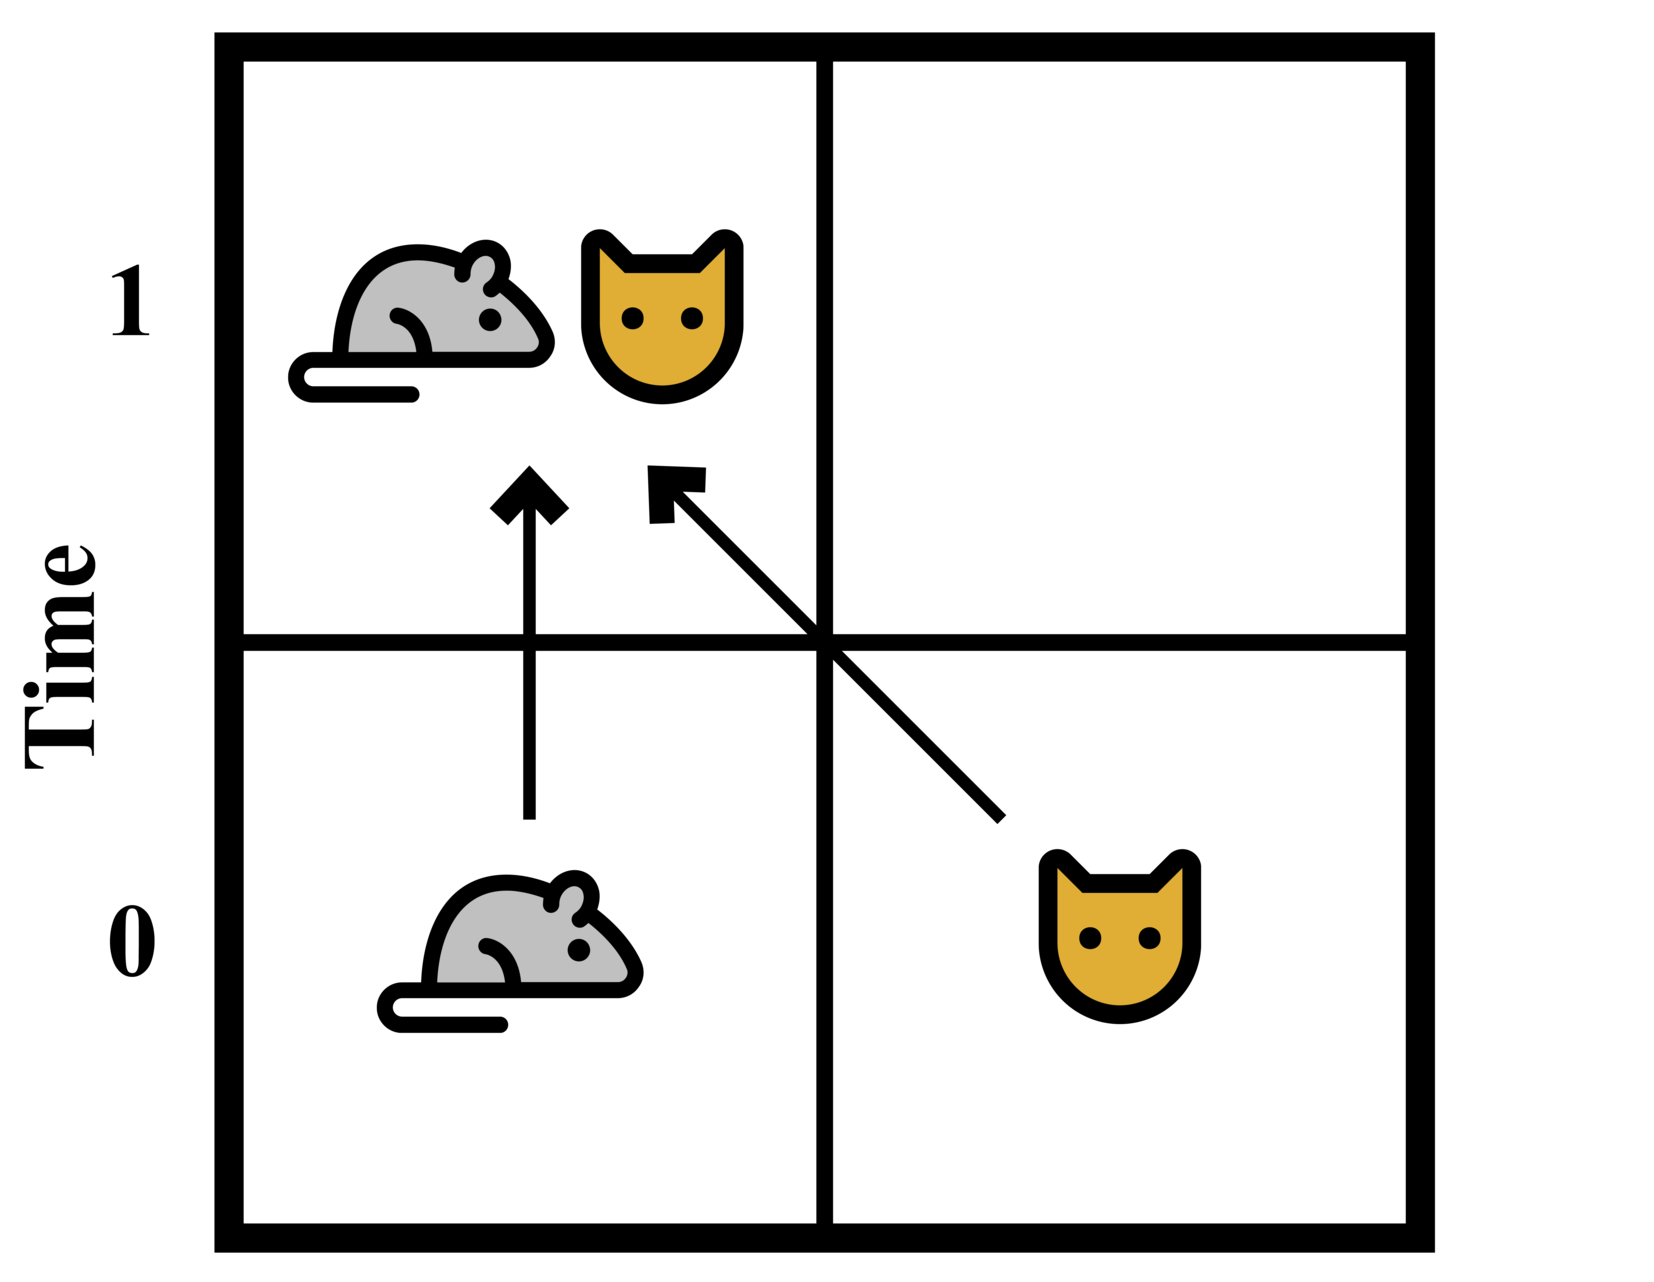
\includegraphics[scale=0.5]{figs/catMouseSm}
	}
	\caption{A simple cat and mouse model.\label{fig:AB-MCMC-1}}
\end{figure}


Let a model timestep be a tensor $E \in \mathbb{R}_{SA}$ whose elements $e_{\psi a}$ are the number of agents in state $\psi$ that perform act $a$ in this timestep. For example, the timestep shown in Figure~\ref{fig:AB-MCMC-1} for the cat and mouse example would be
\[
E = \kbordermatrix{
	& \alpha_0 & \alpha_1 \\
	\sigma_0 & 0 & 0 \\
	\sigma_1 & 1 & 0 \\
	\sigma_2 & 0  & 1 \\
	\sigma_3 & 0 & 0 \\
}
\]
where one agent in state $\sigma_1$ (\textit{right cat}) performs action $\alpha_0$ (\textit{move}) and one agent in state $\sigma_2$ (\textit{left mouse}) performs action $\alpha_1$ (\textit{stay still}).

Let a model trajectory, $T$, be a tensor in $\mathbb{R}^N_{SA}$ that represents $N$ timesteps of a model with $S$ agent states and $A$ actions, so that $T^t_{\psi a}$ denotes the $(\psi, a)^{th}$ element of the $t^{th}$ timestep matrix.

A tensor must satisfy a number of constraints in order to be a valid trajectory of an ABM. Since the elements of a trajectory are counts of agents, they must be non-negative integers. We'll call this the \textit{non-negative integer constraint} and define the set of all non-negative integer tensors
\begin{equation}
\mathbb{N}^N_{SA} = \left\{ T \in \mathbb{R^N_{SA}}: T^t_{\psi a} \ge \mathbf{0}^t_{\psi a}, T^t_{\psi a} \in \mathbb{Z}\right\}
\label{nonNegativeInt}
\end{equation}

A trajectory must also be \textit{continuous} by which we mean that the number of agents in each state at the end of timestep $t-1$ must be the number of agents in each state at the beginning of timestep $t$\footnote{This does not mean that agents cannot leave or enter the system, only that if they do then that change must be defined as part of an action.}. We call this the \textit{continuity constraint} and define the set of continuous tensors, with respect to an action function $F$:
\begin{equation}
\mathcal{C}^N_{SA}(F) = \left\{T\in\mathbb{R}^N_{SA}:  \forall \left(  1 \le \bar t < N\right): F^{\psi a}_{\phi} T^{t-1}_{\psi a} = \mathbf{1}^bT^{t}_{\phi b}\right\}
\label{continuous}
\end{equation}
where $F \in \mathbb{R}^{SA}_S$ is the tensor such that  $F^{\psi a}_* = F(\psi, a)$. Note that this assumes that a timestep is performed by updating all agents in parallel, i.e. agents must act with no information about the actions of other agents in the same timestep. This is different from serial update, where agents are updated in a particular order within a timestep and have access to information about the actions of agents that come before them in the ordering. Note also that this assumes that agents in the same state are indistinguishable, i.e. if we swap two agents in the same state, the trajectory is unchanged.


So, we define the set of trajectories, $\mathcal{T}^N_{SA}(F)$, as set of tensors that satisfy \eqref{nonNegativeInt} and \eqref{continuous}.
\begin{equation}
\mathcal{T}^N_{SA}(F) = \mathbb{N}^N_{SA} \cap \mathcal{C}^N_{SA}(F)
\label{SetOfTrajectories}
\end{equation}


\subsection{The posterior}

Our ultimate goal is to generate samples from the Bayesian posterior over the trajectories, given a set of observations, $\Omega$
\[
P\left(T \middle| \Omega\right) \propto P\left(\Omega \middle| T\right)P(T)
\]
The prior over the trajectory, $P(T)$, can be composed from terms involving the agent timestep function, $\pi(\psi,\Psi,a)$, which gives the probability that a single agent will perform action $a$ given that it starts in state $\psi$ and is surrounded by agents $\Psi$. First consider all the agents that are in state $\psi$ at the beginning of timestep $t$. Let $R\in\mathbb{R}_A$ be a vector whose elements $R_a$ are the number of these agents that perform act $a$ in timestep $t$. The probability distribution of $R$ is just a multinomial distribution
\begin{equation}
P\left(R \mid \Psi, \psi\right) = 
\begin{cases}
\Psi_\psi!\prod_a \frac{\pi(\psi,\Psi,a)^{R_ a}}{R_a!} & \text{ if } R_a\mathbf{1}^a = \Psi_\psi \\
0 & \text{otherwise}
\end{cases}
\end{equation}
If we now let $P(\Psi^0)$ be the prior probability over the number of agents in each state at the beginning of the trajectory then the prior over trajectories can be written 
\begin{equation}
P(T) =
\begin{cases}
P(\Psi^0 = T^0_{* c}\mathbf{1}^c)
\prod_{t, \psi}\left(T^t_{\psi b} \mathbf{1}^b \right)!
\prod_a \frac{\pi(\psi, T^{t}_{* d}\mathbf{1}^d,a)^{T^{t}_{\psi a}}}{T^{t}_{\psi a}!} & \text{if } T \in \mathcal{T}^N_{SA}(F) \\
0 & \text{otherwise}\\
\end{cases}
\end{equation}

The likelihood, $P(\Omega|T)$, can also be decomposed. Without loss of generality, we take $\Omega$ to consist of some number of observations that are independent of each other given the trajectory, so that $\Omega$ is a set of pairs $(\omega,v)$ that consist of a stochastic observation operator $\omega$ and an observed value $v$ (which may be a vector). We write $P(\omega(T)=v)$ to denote the probability of observation operator $\omega$ making observation $v$ on trajectory $T$. So
\[
P(\Omega|T) = \prod_{(\omega,v) \in \Omega} P(\omega(T)=v)
\]
and posterior can be written as
\begin{equation}
P(T|\Omega) \propto 
\begin{cases}
\prod_{(\omega,v) \in \Omega,t, \psi, a}
P(\Psi^0 = T^0_{* c}\mathbf{1}^c)
P\left(\omega(T)=v\right)
\left(T^t_{\psi b} \mathbf{1}^b \right)!
\frac{\pi(\psi, T^{t}_{* d}\mathbf{1}^d,a)^{T^{t}_{\psi a}}}{T^{t}_{\psi a}!} & 
 \text{if } T \in \mathcal{T}^N_{SA}(F) \\
0 & \text{otherwise}\\
\end{cases}
\label{posterior}
\end{equation}

\section{Approximating the support of the posterior}
%##########################################

Sampling from the posterior is difficult because it is hard to find proposal trajectories that have non-zero probability. Our strategy to solve this problem is to first derive an expression for a volume of trajectory space, $\mathcal{P}^N_{SA}$, that contains the support of the posterior, $\supp(P(T|\Omega))$ (the support is just the set of trajectories that have non-zero probability). If we choose $\mathcal{P}^N_{SA}$ so that it is easy to sample from and a relatively tight approximation of $\supp(P(T|\Omega)))$ then there's a good chance that a sample drawn from $\mathcal{P}^N_{SA}$ will have non-zero probaqbility. If a sample has zero probability we simply reject it and sample again.

From equation \eqref{posterior}
\begin{equation}
\begin{aligned}
\supp (P( T |\Omega)) = 
& \bigcap_{(\omega,v) \in \Omega,t, \psi, a} \mathcal{T}^N_{SA} \cap \\ 
&\supp(P(\Psi^0 = T^0_{* c}\mathbf{1}^c)) \cap \\
& \supp\left(P\left(\omega(T)=v\right)\right) \cap \\
&\left( \supp\left(\pi(\psi,T^t_{* b}\mathbf{1}^b,a)\right) \cup \left\{T:T^t_{\psi a} = 0\right\} \right)
\end{aligned}
\label{support}
\end{equation}
i.e. in order for $T$ to have non-zero posterior probability, it must be a trajectory of the ABM, it must have a start state that has non-zero prior probability, all the observation likelihoods must be non-zero and each element of $T$ must denote an agent action with non-zero probability.


\subsection{Convex $\mathbb{Z}$-polyhedra and $\mathbb{Z}$-distributions}
%################################################################
\label{BPoly}

Let a $\mathbb{Z}$-polyhedron be a set of tensors whose elements satisfy a set of linear constraints and belong to the set of integers: 
\[
\mathcal{P^N_{SA}} = \left\{ T\in\mathbb{\mathbb{Z}}^N_{SA} : L^{i} \le  C^{\psi ai}_t T^t_{\psi a} \le U^{i} \right\}
\]
where $C \in \mathbb{Z}^{SAI}_{N}$, $L \in \mathbb{Z}^I$ and $U \in \mathbb{Z}^I$ for some $I$. This is similar to the $\mathbb{Z}$-polyhedron described in \cite{quinton1996manipulating}).

From equation \ref{SetOfTrajectories} we can see immediately that the set of all trajectories, $\mathcal{T}^N_{SA}$, is a  $\mathbb{Z}$-polyhedron. The supports of the prior, $P(\Psi^0)$, the observations, $P(\omega(T)=v)$, and the agent actions, $\pi(\psi,T^t_{*b}\mathbf{1}^b,a)$, can often be easily expressed as $\mathbb{Z}$-polyhedra. However, if this is not the case, each of the probability distributions can be expressed as computer programs. In practice, these computer programs will be simple and it will be possible to use a technique known as \textit{abstract interpretation}\cite{cousot1977abstract} using the domain of convex polyhedra\cite{cousot1978automatic}\cite{becchi2018efficient}\cite{fukuda2020polyhedral} to efficiently calculate a convex polyhedron that contains the support of the program. Software to perform abstract interpretation using convex polyhedra already exists\cite{henry2012pagai}\cite{GN2021}\cite{jeannet2009apron}\cite{bagnara2008parma} and the technique has been used in applications such as compiler optimization\cite{nsjodin2009design} and verification of safety-critical systems\cite{halbwachs1997verification}. The programs may contain calls to a random number generator \texttt{Random()} that returns a random floating-point number $0 \le r < 1$. This can be represented in the polyhedral domain by introducing a new variable, $r$, that satisfies $0 \le r < 1$ for each call to \texttt{Random()}.

If the number of agents is very much smaller than the number of agent states (which is often the case with agent based models) then we may be willing to make the assumption that in any timestep there is at most one agent performing a given action from a given start state (i.e. $\forall \psi, a, t: T^{\psi a}_t \in \{0,1\}$). Under this assumption, which we'll call the \textit{Fermionic assumption}, the set of \textit{Fermionic trajectories}, $\mathcal{F}^N_{SA} = \left\{T\in\mathcal{T}^N_{SA}: \forall \psi, a, t: T^{\psi a}_t \in \left\{0,1\right\}\right\}$, all lie on the corners of the unit hypercube. So the intersection of $\mathcal{F}^N_{SA}$ with any set is a $\mathbb{Z}$-polyhedron and $\supp(P(T|\Omega))$ can always be exactly represented as a $\mathbb{Z}$-polyhedron.

So, if we let $\mathcal{P}^N_{SA}(f)$ be a $\mathbb{Z}$-polyhedron that contains $\supp(f)$ on the integer points then from equation \eqref{support}
\begin{equation}
\begin{aligned}
\supp(P( T |\Omega)) \subseteq \mathcal{P}^N_{SA}(P(T|\Omega)) =
& \bigcap_{(\omega,v) \in \Omega,t,\psi, a} \mathcal{T}^N_{SA} \cap \\
& \mathcal{P}^N_{SA}(P(\Psi^0 = T^0_{* c}\mathbf{1}^c)) \cap\\
&    \mathcal{P}^N_{SA}\left(P\left(\omega(T)=v\right)\right) \cap \\
& 
\left(\mathcal{P}^N_{SA}\left(\pi(\psi,T^t_{* b}\mathbf{1}^b,a)\right)
\cup
\left\{T: T^t_{\psi a} = 0\right\}\right)
\\
\end{aligned}
\label{polyhedralSupport}
\end{equation}

The intersection of two $\mathcal{Z}$-polyhedra is easy to express as another $\mathcal{Z}$-polyhedron by just concatenating the constraints
\begin{multline}
\left\{ T\in\mathbb{\mathbb{Z}}^N_{SA} : L \le C^{\psi a*}_{t} T^t_{\psi a} \le U \right\}
\cap \left\{ T\in\mathbb{\mathbb{Z}}^N_{SA} : L' \le D^{\psi a *}_{t} T^t_{\psi a} \le U' \right\} \\
= \left\{ T\in\mathbb{\mathbb{Z}}^N_{SA} : {L \choose L'}  \le  {C^{\psi a*}_t \choose D^{\psi a*}_t} T^t_{\psi a} \le {U \choose U'} \right\}
\label{intersection}
\end{multline}
so the only difficulty in calculating $\mathcal{P}^N_{SA}(P(T|\Omega))$ from \eqref{polyhedralSupport} is the union in the final term. To transform this into an intersection we introduce an auxiliary variable $z$ and use the identity
\begin{multline}
\left\{ T\in\mathbb{Z}^N_{SA} : L^i \le C^{\phi bi}_{s} T^s_{\phi b} \le U^i \right\}
\cup
\left\{T: T^t_{\psi a} = 0\right\}
=\\
\left\{
T\in\mathbb{Z}^N_{SA}, z\in\{0,1\}:\right.\\
C^{\phi b i}_{s} T^s_{\phi b} + (\overline{B}^i-U^i)z \le \overline{B}^i,\\
\underline{B}^i \le C^{\phi b i}_{s} T^s_{\phi b} + (\underline{B}^i-L^i)z,\\
0 \le uz - T^t_{\psi a},\\
\left. z - T^t_{\psi a} \le 0
\right\}
\label{implication}
\end{multline}
where $u$ is the maximum value that any element of $T$ can take, the elements of $\overline{B}\in\mathbb{R}^I$ are defined as
\[
\overline{B}^i = \frac{u\sum_{s,\phi,b} \left( C^{\phi bi}_{s} + \left|C^{\phi bi}_{s}\right|\right)}{2}
\]
and the elements of $\underline{B}\in\mathbb{R}^I$ are defined as
\[
\underline{B}^i = \frac{u\sum_{s,\phi,b} \left(C^{\phi bi}_{s} - \left|C^{\phi bi}_{s}\right|\right)}{2}
\]

To see why this identity holds, note first that the constraints on $z$ makes it into an indicator variable that is 0 if $T^t_{\psi a}=0$ or 1 otherwise. When $z=1$ the first set of constraints is equal to $C^{\phi bi}_{s} T^s_{\phi b} \le U^i$ and the second is equal to $L^i \le C^{\phi bi}_{s} T^s_{\phi b}$ so their intersection is $L^i \le  C^{\phi bi}_{s} T^s_{\phi b} \le U^i$ as required, whereas when $z=0$ we have the constraints $\underline{B}^i \le C^{\phi bi}_{s} T^s_{\phi b} \le \overline{B}^i$. But $\underline{B}^i$ and $\overline{B}^i$ are lower and upper bounds on the value of $C^{\phi bi}_{s} T^s_{\phi b}$ so this is satisfied for all trajectories, as required.

There are two things worth noting here. Firstly if we make the Fermionic assumption then $z = T^t_{\psi a}$ and the auxiliary indicator variables become unnecessary. Secondly, we must impose a finite value for $u$, the maximum value that elements of the trajectory can take. In practice, this is not a problem as we can give $u$ a value such that the probability of any trajectory of interest having any element larger than $u$ is small.

Using \eqref{polyhedralSupport}, \eqref{intersection} and \eqref{implication} the support of the posterior can be reduced to a $\mathbb{Z}$-polyhedron.

The idea of a $\mathbb{Z}$-polyhedron as the support for a probability distribution naturally leads to the idea of a $\mathbb{Z}$-distribution which is a discrete probability distribution defined over the members of a $\mathbb{Z}$-polyhedron. From the above, it can be seen that the posterior distribution of an ABM trajectory can be expressed as a $\mathbb{Z}$-distribution.

As an illustration, consider a two-timestep trajectory of the cat and mouse model described in section \ref{abmdef}. Suppose we flip a fair coin to decide whether each agent state is occupied or empty at $t=0$. Suppose also that we observe a cat in the left grid-square at time $t=1$. Our aim is to construct a $\mathbb{Z}$-polyhedron, $\mathcal{P}^2_{4\,2}(P(T|\Omega))$, that describes the support of the posterior.

Working through \eqref{polyhedralSupport} term by term, the $\mathcal{T}^2_{4\,2}$ term is just the continuity constraints in \eqref{continuous}, which are already in linear form so we're done. The second term is the support of the prior. This constrains each agent state at $t=0$ to be at most 1, which can be expressed as
\[
\left\{T:T^0_{\psi 0} + T^0_{\psi 1} \le \mathbf{1}_{\psi}\right\}
\]

The third term is the support of the observation. Since we observe a cat in the left grid-square at time $t=1$ we need to add the constraint
\[
T^1_{0 0} + T^1_{0 1} = 1
\]
The final term is the constraint due to agent interactions. The impossible interactions are a mouse staying put when there is a cat on the same gridsquare or moving when there are no cats, which translates to the four cases
\begin{equation}
\begin{aligned}
\supp(\pi(2,T^t_{* a}\mathbf{1}^a,0)) &= \left\{ T: -T^t_{0 0} - T^t_{0 1} \le -1 \right\}\\
\supp(\pi(3,T^t_{* a}\mathbf{1}^a,0)) &= \left\{ T: -T^t_{1 0} - T^t_{1 1} \le -1 \right\}\\
\supp(\pi(2,T^t_{* a}\mathbf{1}^a,1)) &= \left\{ T: T^t_{0 0} + T^t_{0 1} \le 0 \right\}\\
\supp(\pi(3,T^t_{* a}\mathbf{1}^a,1)) &= \left\{ T: T^t_{1 0} + T^t_{1 1} \le 0 \right\}
\end{aligned}
\label{actionConstraints}
\end{equation}
for all t. If, for simplicity, we make the Fermionic assumption by adding the constraints
\[
\mathbf{0}^t_{\psi a} \le T^t_{\psi a} \le \mathbf{1}^t_{\psi a}
\]
then using the identity in \eqref{implication} to take the union of each constraint in \eqref{actionConstraints} with $\left\{T: T^t_{\psi a} = 0\right\}$ finally gives the four constraints
\[
\begin{aligned}
-T^t_{0 0} - T^t_{0 1} + T^t_{2 0} & \le 0\\
-T^t_{1 0} - T^t_{1 1} + T^t_{3 0} & \le 0\\
T^t_{0 0} + T^t_{0 1} + 2T^t_{2 1} & \le 2 \\
T^t_{1 0} + T^t_{1 1} + 2T^t_{3 1} & \le 2
\end{aligned}
\]
for each timestep $t=0$ and $t=1$ to describe the agent interactions.

Taken together, these constraints define a $\mathbb{Z}$-polyhedron that is the set of (Fermionic) trajectories for the cat and mouse ABM, and when combined with equation \eqref{posterior} defines $P(T|\Omega)$ as a $\mathbb{Z}$-distribution.

\section{Sampling from a $\mathbb{Z}$-distribution}
%#################################################

Having shown how to express $P(T|\Omega)$ as a $\mathbb{Z}$-distribution, we now show how to construct a Markov process which will allow us to sample from a $\mathbb{Z}$-distribution.

To do this we need to define
\begin{itemize}
\item a set of Markov states, $\mathcal{M}$

\item a probability measure $P: \mathcal{M} \to \mathbb{R}$ which gives the probability of each Markov state (this need not be normalised, though, as the Metropolis Hastings algorithm only ever needs probability ratios)

\item a stochastic proposal function $f:\mathcal{M} \to \mathcal{M}$ from which we can generate transitions to a new Markov state given the current Markov state

\item a mapping $E:\mathcal{M} \to \mathbb{R}^T_{SA}$ which maps Markov states to trajectories so we can recover the sample.
\end{itemize}

In order to be of use in practice, the proposal function, $f$, must have the following properties:
\begin{itemize}
	\item For any two Markov states there should exist a sequence of transitions which forms a path between those states and has non-zero probability of being proposed.
	
	\item For any proposal from state $S_a \to S_b$ with non-zero probability, the probability of the reverse transition from $S_b \to S_a$ should also be non-zero. This allows us to attain detailed balance in the Metropolis Hastings algorithm. The average ratio of forward and backward probabilities times the ratio of start and end state probabilities should be close to 1 to ensure that a reasonable proportion of proposals are accepted.
	
	\item Given a current Markov state, there should be computationally efficient procedure to generate a proposal and calculate its acceptance probability. 
\end{itemize}


\subsection{The set of Markov states}
%#############################################

Given a $\mathbb{Z}$-polyhedron, we split the constraints into two sets: equalities (i.e. those whose lower and upper bound have the same value) and inequalities (i.e. those whose lower and upper bounds differ):
\begin{equation}
\mathcal{P} = \left\{T \in \mathbb{Z}^N_{SA}: L^i \le C^{\psi ai}_t T^t_{\psi a} \le U^i \cap D^{\psi ai}_t T^t_{\psi a} = E^i \right\}
\label{zPolySupport}
\end{equation}

Suppose there are $N_e$ equality constraints (i.e. $E$ is an $N_e$ dimensional vector of integers) and we partition the elements of $T$ into `basic' and `non-basic' elements, so that there are exactly $N_e$ basic elements and $NSA - N_e$ non-basic elements (note that since the continuity constraints \eqref{continuous} are equality constraints then $N_e \ge (N-1)S$ ).

A partition of a tensor $T$ can be defined as a pair of tensors $Q\in\{0,1\}_{SAN_e}^{N}$ and $R\in\{0,1\}_{SAJ}^{N}$, where $J=NSA - N_e$. $Q$ and $R$ take vectors of basic, $X\in\mathbb{R}^{N_e}$, and non-basic, $Y\in\mathbb{R}^J$, variables and pack them into a trajectory tensor, without changing their values. More formally, $Q$ and $R$ should satisfy
 \[
Q_{\psi ai}^{t} \mathbf{1}^i + R_{ \psi  aj}^{t} \mathbf{1}^j =  \mathbf{1}^t_{\psi a}
 \]
 \[
Q_{\psi ai}^{t} \mathbf{1}_t^{\psi a} = \mathbf{1}_i
 \]
 \[
R_{\psi aj}^{t} \mathbf{1}_t^{\psi a} = \mathbf{1}_j
\]
Given the partition, we can map from a vector of basic variables, $X$ and a vector of non-basic variables, $Y$, to a trajectory
\begin{equation}
T^{t}_{\psi a} =  Q_{\psi ai}^{t} X^i + R_{ \psi  aj}^{t} Y^j
\label{trajXY}
\end{equation}
If we now let
\begin{equation}
B_i^k = D^{\psi ak}_{t}Q_{\psi a i}^{t}
\label{Bmatrix}
\end{equation}
and
\[
N_j^k = D^{\psi ak}_{t}R_{\psi aj}^{t}
\]
then we can write the equality constraints as
\begin{equation}
B_i^kX^i + N_j^kY^j = E^k
\label{eqconstraints}
\end{equation}

Now, since there are $N_e$ basic variables and $N_e$ equality constraints, $B$ is square so if we choose the basic variables in such a way as to ensure that $B$ has an inverse then
\begin{equation}
X^i = (B^{-1})^i_k(E^k + N_j^kY^j)
\label{basicvars}
\end{equation}
inserting this into \eqref{trajXY} gives
\begin{equation}
T^t_{\psi a} =  Q_{\psi ai}^{t}(B^{-1})^i_k(E^k + N_j^kY^j) + R_{\psi aj}^{t } Y^j
\label{markovtotrajectorytensor}
\end{equation}
or equivalently
\begin{equation}
T^t_{\psi a} =  K^t_{\psi a} + M^{t}_{\psi aj} Y^j
\label{markovtotrajectory}
\end{equation}
where
\[
K^t_{\psi a} = Q_{\psi ai}^{t} (B^{-1})^i_kE^k
\]
and
\[
M^{t}_{\psi aj} = Q_{\psi ai}^{t} (B^{-1})^i_kN_j^k + R_{\psi aj}^{t}
\]
If we also choose the basic variables such that all elements of $B^{-1}$ are integer then we can define the set of Markov states to be
\[
\mathcal{M} = \left\{ Y \in \mathbb{Z}^J: \forall i:0 \le Y_i \le u \right\}
\]
where $u$ is the upper limit on the occupancy of agent actions, and map each Markov state, $Y$, to a unique integer trajectory using \eqref{markovtotrajectory}.

\subsection{The probability of a Markov state}

Given a Markov state, $Y$, that satisfies $0 \le Y_j \le u$, the associated trajectory given by equation \eqref{markovtotrajectory} is guaranteed to satisfy all the equality constraints. However, there is no guarantee that the basic variables given by eq \eqref{basicvars} will be within their bounds or that the inequality constraints will be satisfied. To deal with this we introduce the concept of \textit{infeasibility} which is a measure of the extent to which a Markov state fails to satisfy the inequality constraints.

Given the inequality constraints of the $\mathbb{Z}$-distribution (including the upper and lower limits of the trajectory elements themselves)
\[
L^i \le C^{\psi ai}_{t} T^t_{\psi a} \le U^i
\]
using \eqref{markovtotrajectory} this can be written as
\begin{equation}
L^i \le J^i + Q_j^i Y^j \le U^i
\label{ineqconstraints}
\end{equation}
where
\[
J^i = C^{\psi ai}_{t} K^t_{\psi a}
\]
and
\[
Q_j^i = C^{\psi ai}_{t}M^{t}_{\psi aj}
\]

let the infeasibility of the $i^{th}$ constraint, $\iota(Y)_i$, be defined to be equal to 0 if the constraint is satisfied or equal to the distance to the nearest bound otherwise
\[
\iota(Y)_i =
\begin{cases}
L^i- J^i - Q_j^iY^j & \text{if }J^i + Q_j^iY^j<L^i\\
J^i + Q_j^iY^j-U^i & \text{if }J^i + Q_j^iY^j>U^i\\
0 & \text{otherwise}
\end{cases}
\]
and let the total infeasibility be the sum of infeasibilities of all constraints
\[
\iota(Y) = \sum_i \iota(Y)_i
\]
So, each Markov state is associated with a total infeasibility with respect to the inequalities of the $\mathbb{Z}$-distribution. 

If the infeasibility is zero, then all the constraints are satisfied and the probability is defined to be proportional to the probability of the $\mathbb{Z}$-distribution
\[
P(Y) \propto P(K^t_{\psi a} + M^{t}_{\psi aj}Y^j)
\]

If the infeasibility is not zero, then the probability is defined in the following way. Given an upper bound on the trajectory's elements, $u$, we define the \textit{clamped} trajectory
\[
\overline{\underline{T^t_{\psi a}}} = 
\begin{cases}
0 & \text{if }T^t_{\psi a}<0\\
u & \text{if }T^t_{\psi a}>u\\
T^t_{\psi a} & \text{otherwise}
\end{cases}
\]

Furthermore, let $H_t^{\psi a}$ be a log-linear approximation to the target $\mathbb{Z}$-distribution so that for feasible trajectories
\[
H_t^{\psi a}T^t_{\psi a} \approx \log(P(T))
\]
For infeasible trajectories, we define the probability, $P_\iota$, as
\begin{equation}
\log(P_\iota(Y)) = H_t^{\psi a}\overline{\underline{K^t_{\psi a}+M^{t}_{\psi aj}Y^j}} - \frac{\iota(Y)}{\tau} + A
\label{loglinprob}
\end{equation}
where $\tau$ is a tunable parameter and $A$ is a normalisation constant.

This means that infeasible states have non-zero probability and the Markov chain will pass through some infeasible states.  However, if we just ignore these and only take samples from feasible states then we end up with samples from the target $\mathbb{Z}$-distribution. Allowing the Markov chain to pass through infeasible states has the advantage of ensuring that there exists a path between any two feasible states and improves mixing. The price we pay for this is the computational cost of moving through infeasible states that don't generate useful samples.

If we define the \textit{energy} of a Markov state to be
\[
E(Y) =
\begin{cases}
-\tau log(P(Y)) & \text{if }  \iota(Y) = 0\\
\iota(Y) - \tau H_t^{\psi a}\overline{\underline{K^t_{\psi a}+M^{t}_{\psi aj}Y^j}} & \text{otherwise}
\end{cases}
\]
then the probability of a Markov state can be written in the form
\begin{equation}
P(Y) \propto e^{\frac{-E(Y)}{\tau}}
\end{equation}
This is the form of a Boltzmann distribution which describes a thermodynamic system at equilibrium with a heat bath of ``temperature'' $\tau$. It has been shown that simulations of thermodynamic systems of this type are able to solve large integer optimisation problems \cite{kirkpatrick1983optimization}. In our case, we don't need to change the temperature during the sampling process, but we do need to choose a value for $\tau$. Higher temperatures will increase mixing in the Markov chain, but will also increase the proportion of time spent in infeasible states so we need to find a temperature that is high enough to ensure good mixing of the chain but low enough to ensure a reasonable proportion of samples are feasible. We have found that a good rule of thumb is to set the temperature so that 50\% of the samples in a chain are infeasible.

\subsection{Transitions between Markov states}

Given a Markov state, we transition to another state by choosing an element of  $Y$ and perturbing it by $\pm 1$. If the element begins on one of its bounds then the out-of-bound perturbation is wrapped around to the opposite bound). This defines the set of transitions between Markov states. Let the set of all Markov states reachable from state $Y$ be denoted by $\mathcal{D}(Y)$. 

\subsubsection{The probability of transitions}

The probability of a proposed transition from $Y$ to $Y'$ is defined to be
\[
P(Y \to Y') = \frac{\min\left(1, \frac{P_\iota(Y')}{P_\iota(Y)}\right)}{S(Y)} 
\]
where $P_\iota$ is the log-linear probability defined in \eqref{loglinprob} and
\[
S(Y) = \sum_{Y'\in \mathcal{D}(Y)}\min\left(1, \frac{P_\iota(Y')}{P_\iota(Y)}\right)
\]
Note that this is irrespective of whether $Y$ or $Y'$ are feasible.

Given this, the Metropolis-Hastings acceptance probability is
\[
\alpha = \frac{P(T')P(Y' \to Y)}{P(T)P(Y \to Y')} = 
\frac{P_\iota(Y)}{P(Y)} \frac{P(Y')}{P_\iota(Y')}  \frac{S(Y)}{S(Y')}
\]

When $Y$ is infeasible $\frac{P_\iota(Y)}{P(Y)} = 1$. When $Y$ is feasible $P_\iota(Y)$ approximates $P(Y)$ so their ratio should be close to 1. Finally, $S(Y)$ will not change very much between transitions so the ratio $ \frac{S(Y)}{S(Y')}$ should also be close to 1 meaning that the acceptance probability should also be close to 1.

\subsection{Choosing a basis}

The definition of the Markov chain depends on a partition of the trajectory into basic and non-basic variables such that $B$ in equation \eqref{Bmatrix} has an integer inverse $B^{-1} \in \mathbb{Z}^{N_e}_{N_e}$. In general there exist many possible partitions so it remains to define a method of choosing one. The choice we make affects the way Markov states are mapped to trajectories via equation \eqref{markovtotrajectory} and how infeasibility is calculated via equation \eqref{ineqconstraints}, where the columns of $Q$ can be thought of as basis vectors in a \textit{constraint space} and $Y$ as a coordinate on the grid formed by that basis. The Markov chain can be seen as a random walk around this grid. If we choose a basis that consists of very dense basis vectors then the Markov states adjacent to a feasible trajectory are likely to have high infeasibility and low probability, leading to slow mixing of the chain, so we aim to choose a basis that has sparse basis vectors in the constraint space. This has the additional advantage that when we transition between adjacent Markov states, the probability distribution over transitions changes in only a few dimensions. This means we can use a binary tree to efficiently update and draw from the probability distribution over transitions\cite{TangMutableCategorical}.

Starting with a $\mathbb{Z}$-polyhedron expressed in the form
\[
\mathcal{P} = \left\{T \in \mathbb{Z}^N_{SA}: L^i \le C^{\psi ai}_t T^t_{\psi a} \le U^i \cap D^{\psi ai}_t T^t_{\psi a} = E^i \right\}
\]
suppose we begin with no basic variables so that $R$ is an arbitrary ordering of the elements of a trajectory
\[
T^t_{\psi a} = R^t_{\psi a j}Y^j
\]
If we let
\[
W^*_j = {D^{\psi a*}_t R^t_{\psi aj} \choose C^{\psi a*}_t R^t_{\psi aj}}
\]
and
\[
F = {E \choose \mathbf{0}}
\]
then
\begin{equation}
\mathcal{P} = \left\{T \in \mathbb{Z}^N_{SA}: {\mathbf{0} \choose L} \le W Y - F \le {\mathbf{0} \choose U} \right\}
\label{jointconstraints}
\end{equation}

We use a greedy algorithm to eliminate variables from $Y$ and equality constraints from $W$ one at a time until $N_e$ variables and all equality constraints have been eliminated. The remaining variables in $Y$ will make up the non-basic variables and the remaining constraints will define a basis in the constraint space.

Given a set of constraints in the form \eqref{jointconstraints}, if we choose an element $W^i_j$ to be a \textit{pivot point} such that $W^i_j = \pm1$ and $i < N_e$, we can eliminate variable $Y^j$ and the equality constraint $W^*_i$ by performing Gaussian elimination on the $j^{th}$ column of $W$ and removing row $i$ and column $j$ from $W$, so that
\[
{\mathbf{0} \choose L} \le GWH\hat{Y} - GF \le {\mathbf{0} \choose U}
\]
where $G\in \mathbb{Z}^{N_e-1}_{N_e}$
\[
G =  
\begin{pmatrix}
1 &  & &-\frac{W^0_j}{W^i_j} & & &\\
& \ddots & &\vdots & & &\\
& & 1 & -\frac{W^{i-1}_j}{W^i_j} & & &\\
& &  & -\frac{W^{i+1}_j}{W^i_j} & 1 & &\\
& & & \vdots & & \ddots &\\
& & & -\frac{W^n_j}{W^i_j} & & &1\\
\end{pmatrix}
\]
$\hat{Y}$ is $Y$ with the $j^{th}$ element removed and $H$ is the identity matrix with the $j^{th}$ column removed. Letting $\hat{W} = GWH$ and $\hat{F} = GF$ recovers the canonical form
\[
{\mathbf{0} \choose L} \le \hat{W}\hat{Y} - \hat{F} \le {\mathbf{0} \choose U}
\]

Since $W^i_j = \pm1$, $B^{-1}$ exists and is integer, so $\hat{Y}$ maps to a unique integer trajectory, as required.

Note that $WG$ differs from $G$ in $(\left|G^*_j\right|_0-1)(\left|G^i_*\right|_0-1)$ elements, where $\left|\cdot\right|_0$ is the number of non-zero elements in a tensor. So, this gives an upper bound on the increase in L0-norm, $\left|WG\right|_0 - \left|G\right|_0$ and so gives a measure of how much sparsity may be lost by pivoting on $W^i_j$.  It has been found that choosing $W^i_j$ to be the element that minimises this measure (known as the Markowitz criterion) is a computationally efficient way of maintaining the sparsity of a matrix while performing Gaussian eliminatination\cite{markowitz1957elimination}\cite{maros2002computational}\cite{suhl1990computing}. So, in order to find a sparse basis we choose the element that minimises $(\left|G^*_j\right|_0-1)(\left|G^i_*\right|_0-1)$, perform the elimination and repeat until no more equality constraints remain, $N_e=0$.

\section{Spatial predator-prey demonstration}

We demonstrate the above techniques on a 32x32 grid of ``predator'' and ``prey'' agents. At each timestep a prey agent either moves to an adjacent grid-square (i.e. up, down, left or right with equal probability), dies or gives birth to another prey agent on the an adjacent grid-square. Predators also either move to an adjacent grid-square, die or give birth. However, predators only give birth when there is at least one prey on an adjacent grid-square. In addition, if a prey has any predators on adjacent grid-squares there is a chance it may be eaten. The probability of each behaviour is shown in table \ref{rates}.

\begin{table}
	\begin{center}
		\begin{tabular}{llllc}
		\hline
		Aget type & Adjacent agents & Behaviour & Probability\\
		\hline
		Prey & No predators & die &        0.100\\
			& & give birth &        0.156\\
			& & move &        0.744\\
			& &&\\
		Prey & Predators > 0 & die &        0.100\\
			& & give birth &        0.156\\
			& & be eaten &        0.300\\
			& & move &        0.444\\
			& &&\\
		Predator  & No prey & die  &      0.100\\
			& & move &        0.900\\
			& &&\\
		Predator  & Prey > 0 & die  &      0.100\\
			& & give birth &        0.300\\
			& & move &        0.600\\
		\hline& 
		\end{tabular}
	\end{center}
	\caption{The probabilities of each behaviour in the predator-prey model}
	\label{rates}
\end{table}

\begin{figure}
	\centering
	\resizebox{0.5\textwidth}{!}{
		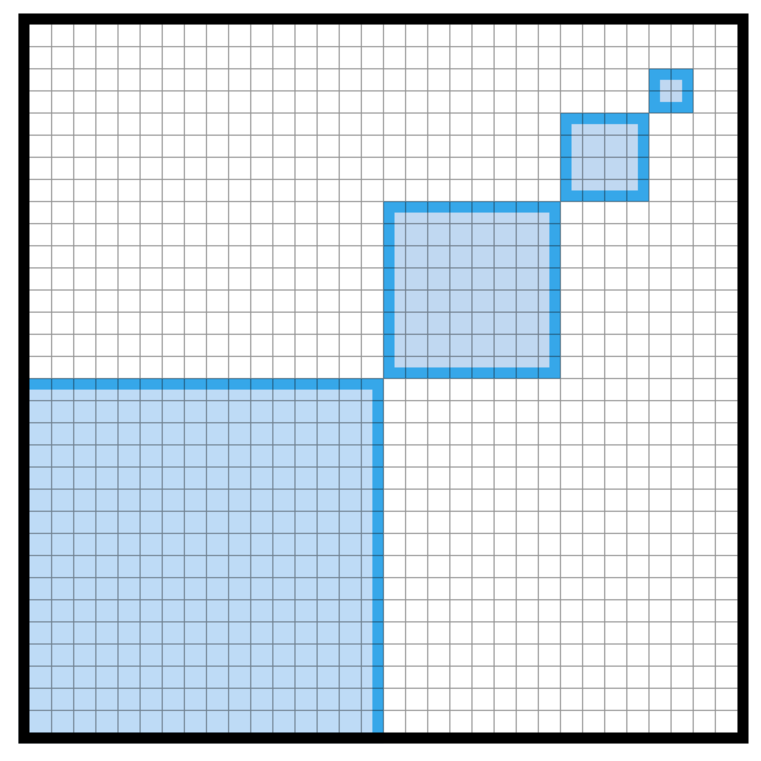
\includegraphics[scale=0.5]{figs/gridRegionsSm.png}
	}
	\caption{Summary statistics consist of the total number of agents in each of the four shaded regions.}
	\label{figRegions}
\end{figure}

\begin{figure}
	\centering
	\resizebox{0.8\textwidth}{!}{
		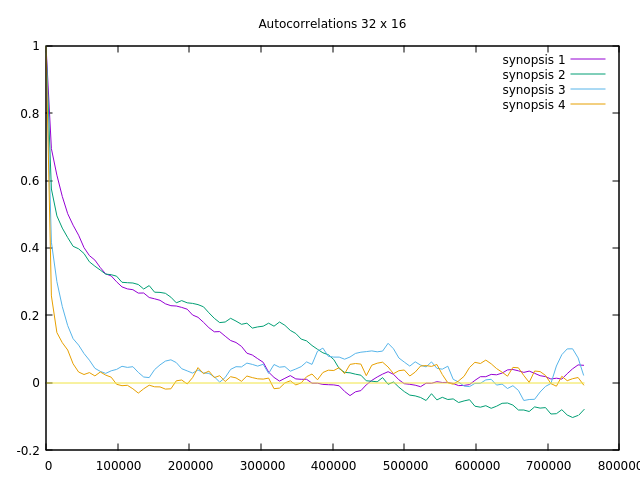
\includegraphics{figs/PredPrey32-16-graph.png}
	}
	\caption{Mean autocorrelation for each scalar of the summary statistics, averaged over all chains.}
	\label{figAutocorrelation}
\end{figure}

\begin{figure}
	\centering
	\resizebox{0.8\textwidth}{!}{
		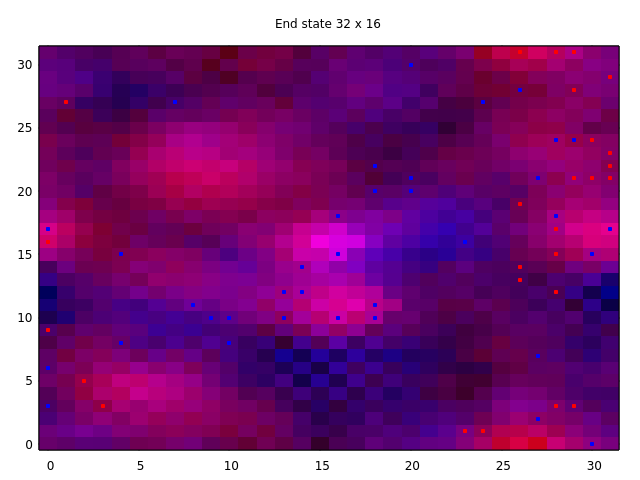
\includegraphics{figs/PredPrey32-16-map.png}
	}
	\caption{Mean number of agents in each gridsquare after the last timestep, averaged over all samples. Blue represents predator, red represents prey. The dots represent the final positions of agents in the simulation from which the observations were generated. The background colour of each square has red/blue intensity proportional to the log of the mean number of prey/predators in that square, respectively.}
	\label{figEndState}
\end{figure}


Simulated observation data was generated by profroming a forward simulation of the model. The number of predators and prey in each gridsquare at the start of the simulation was drawn from a Poisson distribution with rate parameter $\lambda = 0.05$. The model was then simulated forward for 16 timesteps. At each timestep, each gridsquare was observed with a probability of 0.02. If an observation was made, the number of predators in the gridsquare was observed. In order to demonstrate assimilation with observational noise, each predator was observed with probability 0.9 (i.e. the number observed was drawn from a Binomial distribution. Note that our algorithm can also assimilate observations with no noise). The same procedure was then repeated for prey.

Four separate Markov chains of 1,500,000 samples each were generated from the posterior using the method described above. The start state for each chain was drawn from the prior (i.e. model trajectory without any observations). The first 200,000 samples of each chain were discarded and the remaining samples were split into first and last halves to give 8 sample sequences in total. 

In order to assess the convergence of the chains, a set of summary statistics were calculated for each sample of each chain. The summary statistics consisted of the total number of agents within the shaded regions shown in figure \ref{figRegions} measured after the last timestep of the trajectory. This arrangement of regions was chosen in order to capture the convergence at different spatial scales. From the summary statistics, we calculated the the Gelman-Rubin diagnostic \cite{gelman1992inference}, and approximated the autocorrelation at various time lags. Using the notation $x_{ij}$ to refer to a scalar statistic of the $i^{th}$ sample of the $j^{th}$ sequence, given $m$ sequences of $n$ samples each, let $\bar{x}_j$ be the mean of the $j^{th}$ sequence and $\bar{x}$ be the mean over all sequences
\[
\bar{x}_j = \frac{1}{n}\sum_{i=1}^n x_{ij}, \bar{x} = \frac{1}{m}\sum_{j=1}^m \bar{x}_j
\]
let $W$ be the within-sequence variance
\[
W = \frac{1}{m} \sum_{j=1}^m \frac{1}{n-1} \sum_{i=1}^n (x_{ij} - \bar{x}_j)^2
\]
and $B$ be the between-sequence variance
\[
B = \frac{n}{m-1}\sum_{j=1}^m (\bar{x}_j - \bar{x})^2
\]
Following\cite{gelman2013bayesian}, an overapproximation of the true variance of the statistic can be calculated as
\[
\widehat{\text{var}}^+ = \frac{n-1}{n}W + \frac{1}{n}B
\]
and the Gelman-Rubin statistic can be defined as
\[
\hat{R} = \sqrt{\frac{\widehat{\text{var}}^+}{W}}
\]
This gives a measure of the uncertainty in the standard deviation of the statistic due to the fact that we have only taken a finite number of samples. If this number is close to 1, then we have some justification in believing that we have taken enough samples.

Also following\cite{gelman2013bayesian}, we approximated the autocorrelation as
\[
\hat{\rho}_t = 1 - \frac{V_t}{2\widehat{\text{var}}^+}
\]
where
\[
V_t = \frac{1}{n-t} \sum_{i=1}^{n-t} (x_i - x_{i+t})^2
\]

Figure \ref{figAutocorrelation} shows $\hat{\rho}_t$ as a function of $t$ for each scalar in the summary statistics. A decline of $\hat{\rho}_t$ to zero long before $t$ reaches the total number of samples, shows good convergence of the chain. The rate of this decline can be used to calculate the effective number of samples, defined as
\[
\hat{n}_e = \frac{mn}{1 + 2\sum_{t} \hat{\rho}_t}
\]
where the sum runs until $\hat{\rho}_t \le 0$. This approximates of the number of samples from a perfect IID sampler that would give the same uncertainty in the mean of the statistic.

Finally, figure \ref{figEndState} shows the mean number of agents at the end of the simulation, averaged over all samples. This is a visual way of showing that the observations have given rise to a posterior that gives some information about the true positions of the agents.

[Show convergence with problem size/number of constraints or with grid-size / number of timesteps (number of agents?)]

\section{Discussion} 
\label{discussion}
 The technique described here could easily be extended to the problem of parameter estimation by replacing all distributions over the model trajectory with the joint distribution over parameter values and model trajectory and treating our prior beliefs about the parameters as a boundary condition. We can then sample from the joint distribution of parameters and trajectory which, after removing the trajectory, gives a probability distribution over parameter space. If we have observations that span multiple, independent observed time periods, a single parameter distribution can be generated by taking the product of the distributions from the individual time periods.
 
[explain turnaround options, depending on nature of the model: variational, kernel density estimation, particle as known start state, relationship to SMC/particle filtering]

[explain model imperfection: model uncertainty should be included in stochasticity and parameters. Making models that don't fit observation and then making them `almost' fit is a bad strategy. If your model doesn't fit observation, your model assumptions are wrong.]

[explain extension to parameter estimation]

\section{Limitations and further work}

[Under what circumstances can agent behaviour be approximated by convex polyhedron? If agent solves an NP complete problem then the delta PMF must map to a sparse polyhedron, for example]

[column generation for ABMs with larger agent state]

[automatic linearisation from ABM expressed as computer program]

[extension to PPL]

[automated temperature setting]

\section{Conclusion}

We have described and demonstrated an algorithm to sample model trajectories from the posterior distribution of an agent based model given a set of observations. This allows us to use ABMs to perform inference about unobserved variables given a set of observations and to make forecasts given observations up to the present.

As presented, the algorithm is not applicable to agents that have a large amount of internal state (above a few bytes) but we suggest ways that this algorithm can be extended to apply in these cases.

Data assimilation with agent based models is currently in its infancy, and more powerful techniques for performing Bayesian inference with ABM could transform the usefulness and applicability of these models. The 

%\bibliographystyle{unsrtnat}
%\bibliographystyle{apalike} 
\bibliographystyle{apacite}
\bibliography{references}

\end{document}
